% !TEX encoding = UTF-8 Unicode
% !TEX program = pdflatex
% !TEX spellcheck = en_US


% In order to correctly compile this document,
% execute the following commands:
% 1. pdflatex
% 2. pdflatex
% 3. pdflatex



\documentclass[amsthm,ebook]{saparticle}

% IF YOU USE PDFLATEX
\usepackage[utf8x]{inputenc}
% if you write in english and in greek
\usepackage{ucs}
\usepackage[greek,english]{babel}
\languageattribute{greek}{polutoniko}

% IF YOU USE XELATEX
%\usepackage{polyglossia}
% if you write in italian
%\setmainlanguage{italian}
% If you want put some ancient greek:
%\setotherlanguage[variant=polytonic]{greek}
%\newfontfamily{\greekfont}[Ligatures=TeX]{Palatino Linotype}

% dummy text (remove in a normal thesis)
% remove if not necessary
\usepackage{siunitx}
%Natbib for bibliography management
\usepackage[authoryear]{natbib}
% custom commands
\newcommand{\bs}{\textbackslash}

%%%%%%%%
%TITLE:%
%%%%%%%%
\title{Trismegistos Places, a geographical index for all Latin inscriptions}
\author[KUL]{Herbert Verreth\corref{first}}
\address[KUL]{Trismegistos Project, Katholieke Universiteit Leuven, Belgium}
\cortext[first]{Corresponding author. Email: Herbert.Verreth@arts.kuleuven.be}
\date{2015-11-15}
\begin{document}

\maketitle
\begin{abstract}
The Trismegistos database has recently created a geographical index for all Latin inscriptions. For the moment we have
67.820 geographical references attested in Latin documentary texts, but this rough starting material still has to be
refined. This paper describes how we undertook this task, which problems we encountered while doing so, and the choices
we made for the presentation of the material.
\end{abstract}
\keywords{Imperium Romanum, Latin, epigraphy, topography, geography, Trismegistos.}


\noindent The Trismegistos (TM) database (\url{http://www.trismegistos.org}) of the Katholieke Universiteit Leuven in Belgium
gathers the metadata for all documentary and literary texts from Egypt and the Ancient World in general written in
whatever language or script between 800 BC and 800 AD. In this respect we try to collaborate as much as possible with
other scientific databases all over the world. We started some ten years ago with the papyrological material from Egypt
(both Greek and Egyptian), and the last few years - through the collaboration with EAGLE - we have also been
incorporating Latin epigraphical texts from the whole Roman word. For the moment TM shows the metadata for 479.629
texts, 306.925 of them written in Latin or containing Latin passages, but the number keeps on growing. Our direct EAGLE
partners Epigraphic Database Heidelberg (EDH), Epigraphic Database Roma (EDR), Hispania Epigraphica Online Database
(HEp) and Epigraphic Database Bari (EDB) mainly focus on inscriptions on stone and other important texts from the
regions they cover, but they usually omit the inscriptions and stamps on instrumentum domesticum or other minor
materials. Since TM also wanted to incorporate these texts, we were glad to find them in the Epigraphik-Datenbank
Clauss-Slaby (EDCS), which contains virtually all published Latin inscriptions, to fill in the missing gaps, a process
which is still going on.

 Trismegistos is a relational database created within the computer program Filemaker (with as latest version
Filemaker Pro 14). Its contents are uploaded weekly to an online MySQL / PHP environment. Attached to the main TM Text
file are numerous other files, such as Collections, Archives, People, Names and Places. These files automatically copy
the relevant information for every card from the main file, so that no double work is needed. With the help of the
Papyrological Navigator (PN) (\url{http://www.papyri.info}) we developed a PHP environment with the assistance of a
programmer (Jeroen Clarysse), to tag all words starting with a capital occurring in the published papyrological texts,
which yielded in the end a full index of all personal names and toponyms in every Greek and Latin papyrus. This process
is nowadays called Named-Entity Recognition [NER]\footnote{ For more information on NER, \citet[304-313]{BrouxDepauw2}.}. These
TM files within People and Places are freely accessible online and can be looked up, questioned and investigated in a
number of ways. But that is a different story. Here we want to focus on our project to do the same for all published
Latin inscriptions.


 The main credits for the whole set-up of this new project go to Mark Depauw, the Trismegistos director. The general
idea remained the tagging of all words starting with a capital, but this time Depauw tried a new approach, which was
completely imbedded within Filemaker. Since the Roman 'tria nomina' hardly occur in the Greek papyri, also a new
onomastical structure had to be devised for the automatic recognition. As a test case we choose the full text corpus of
the EDCS. All these texts were 'cut up' in capital clusters, i.e. strings of consecutive words all starting with a
capital. Words as \emph{filius}, \emph{nepos} and \emph{libertus} were added to the string so that in most cases the full identification of
a person could be grouped together, e.g. \emph{Quintus Caecilius Quinti filius Quirina Mustacus} (TM 332260), \emph{Caio Annioleno
Cai filio Arnensi Karthaginiensi Galliano} (TM 349961) or \emph{Maesiaes Cai libertae Chrysidis} (TM 244384). A minor
disadvantage of this corpus was the capitalization of the first word of every inscription (which is not done in the
PN), which yields quite a significant number of mere nouns in the group of expected personal names and toponyms. Also
other words starting with a capital were not our prime goal: names of gods, religious festivals, months, army units,
ships, animals, mythological persons and Roman numbers. Excluded (for the moment) are also the names of the emperors
and the members of the imperial family, often occurring in a complicated titulature which is not easy to standardise.
In the end this yielded 898.134 capital cluster cards. From our previous projects we already had a fairly elaborated
reference corpus of Roman personal names, which was now expanded and used by Depauw to match every word in the capital
clusters with the names in the reference corpus. If there was a match, the case of the ending was added, e.g.

\begin{table}[htp]
\begin{center}
\begin{tabular}{ccccccc}
Caio & Annioleno & Cai & filio & Arnensi & Karthaginiensi & Galliano\\
dat & dat & gen & filius & tribus & origo & dat\\
\end{tabular}
\end{center}
\label{Example}
\end{table}%

\begin{figure}[!hbp]
\centering
 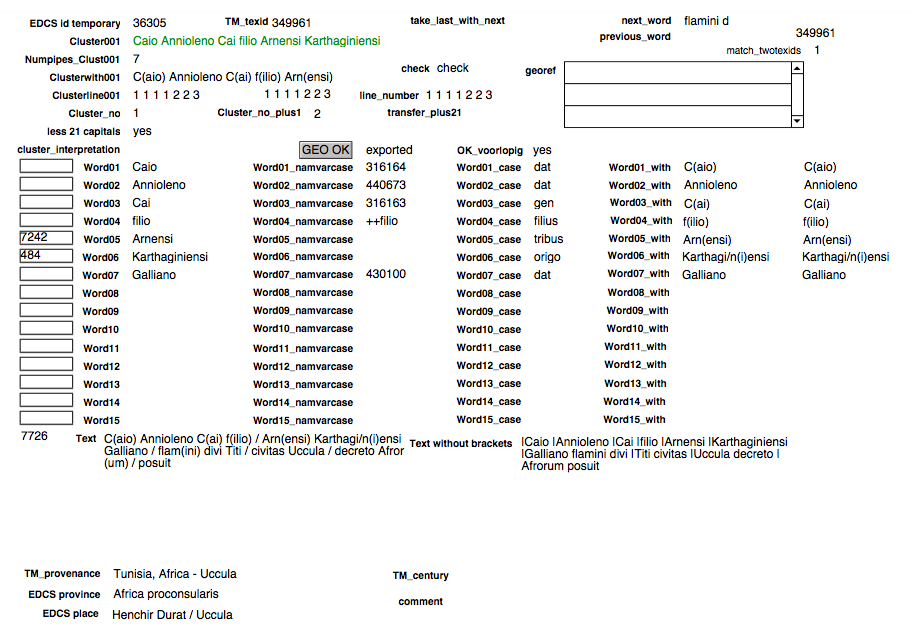
\includegraphics[width=\columnwidth]{EAGLE2016FullPaperVerreth-img001.png}
\caption{Named Entity Recognition with FileMaker Pro 14}
\label{fig:1}
\end{figure}
 




The technical details of this complicated process are better discussed by Depauw himself at some other occasion. On the
basis of this matching all capital cluster cards were split up in two groups: (1) 'yes', this card contains a personal
name [454.183], and (2) 'no', this card does not contain a personal name [443.951]. Within the second group also other
labels have been added, e.g. army [23.201], god [15.663], emperor [41.944], which will be useful for future research.

This is also the phase where the toponyms come in (which can occur both in the first and in the second group).
Within the EAGLE project we created already a fairly large reference corpus for toponyms from the Roman empire, but
this corpus was enlarged by entering the toponyms occurring in the \emph{Itinerarium provinciarum Antonini Augusti} [3.434]
and the \emph{Tabula Peutingeriana} [3.287]. The TM Geo file now contains 46.277 toponyms from all over Egypt and the Roman
empire, both ancient and modern, which cover most of the places where ancient texts have been found, and most of the
toponyms mentioned in Egyptian papyrological and Latin epigraphical sources.\footnote{ For more information on TM Geo,
\citep{verreth2013}.} We played with the idea of automatic matching, like we did for the personal
names, but except for the case of the relatively straightforward tribus names, this yielded no satisfactory results. A
lot of toponyms resemble personal names (e.g. \emph{Florentia}, \emph{Venusia}, \emph{(Fundus) Bassianus}), and the automated identification
of strings such as \emph{Colonia Ulpia Traiana Augusta Fidelis Lepcis Magna }(TM 198383) or \emph{Municipium Augustum Hipponiensium
Regiorum} (TM 200133) seemed too cumbersome. In the end, we settled for plan B, which shows that in `Digital
Humanities', the human component is still essential: we had to go through all 900.000 capital cluster cards manually,
identifying the toponyms in every cluster, adding the corresponding TM Geo number and - whenever necessary - correcting
the indications for yes/no and the automatic identification of the cases of the personal names. It was six months of
tedious work, resulting in 61.139 capital clusters with at least one toponym. No doubt some toponyms escaped our
attention, but we do hope to have identified the majority of the names involved. In this process, however, we also
encountered some set backs, especially in the longer texts and in the more complicated wooden or metal tablets: in the
beta version on which we worked, the creation of the capital cluster strings was not always so perfect as we had hoped
for, and also the line numbers automatically assigned to each cluster string have sometimes gone astray. Mark Depauw is
developing a new and improved version, especially in preparation for the much larger batch of personal names, where it
is virtually impossible to manually correct everything that has gone wrong. Due to these problems I guess that we now
have about only 80 to 90 \% of the toponyms occurring in all Latin inscriptions, but on the whole we are quite pleased
with the result and in due time the remaining toponyms no doubt will find their way into the database also.

Phase 1, the identification of toponyms in the capital cluster strings, was finished in the beginning of July 2015,
and we have now entered phase 2, the incorporation of the capital cluster file into the `real' TM Georef file. For
every place listed in TM Geo we try to list all the ancient text references where that place is attested. The file of
these geographical references (TM Georef) is directly linked with the main TM Text file, so that every reference
automatically receives a chronological and a geographical context. Every toponym found in the capital cluster file is
exported to a separate Georef card. When a toponym exists out of several consecutive elements, like the \emph{colonia} and
\emph{municipium} examples mentioned before, they are automatically grouped on one card. Twofold toponyms such as `\emph{Bythina et
Ponthus'}, which cannot belong to the same capital cluster string because of the intermediary `\emph{et}', are exported double
and then afterwards joined manually. For the moment TM Georef lists 67.820 geographical references attested in Latin
documentary texts and 10.474 references attested in Latin literary texts (but except for Egypt the latter have not yet
systematically been entered). The Latin references make out almost 40 \% of the total of 196.794 Georef cards.




\begin{figure}[!hbp]
\centering
 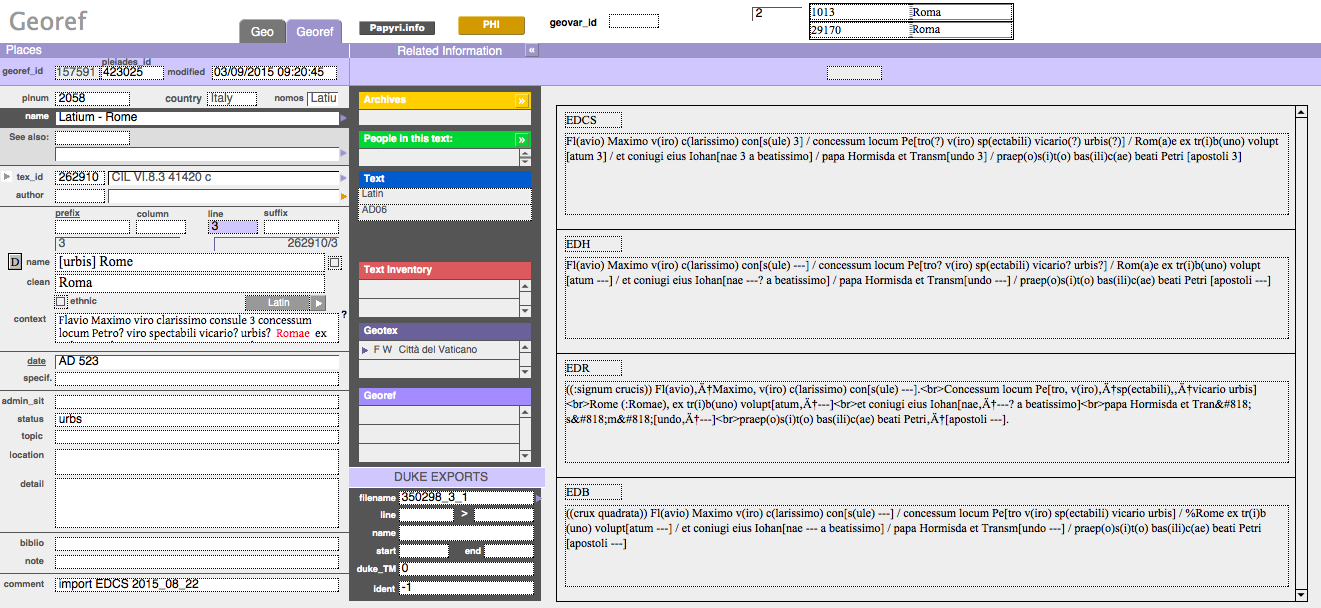
\includegraphics[width=\columnwidth]{EAGLE2016FullPaperVerreth-img002.png}
\caption{The Georef Card}
\label{fig:2}
\end{figure}





In this phase we also start comparing the reading of the toponym in EDCS with the readings of the same passage in
EDH, EDR, HEp and EDB, which can all be shown simultaneously in the Filemaker database. In theory it is possible to
automatically look for differences in readings among all these databases, but because each of them has its own
approach, there will be so many small differences in line numbering, punctuation, the use of uncertainty dots and the
way unconventional spelling in an inscription is indicated, that we doubt that there will be many exact matches. We
therefore think that it will not be worth the enormous amount of work that it would involve. Human observation is again
the answer and we do hope that our partners and the users of the geographical index will point out to us any mistakes
we have made or obsolete readings we have kept. For the online version we have to talk with our partners whether they
want to have their texts also shown on the TM page (like TM does for the texts from PN) or not. For the Open Access
CC-0 texts in the Europeana EAGLE portal, this will in any case be implemented in the future. Anyway it is always
possible to put a direct link on the Georef page to every partner that has the text in its corpus.


Since the users of TM must be able to look for specific spelling variants of each toponyms, all these references are
presented the way they are on the stone, with as little additions or emendations as possible, except of course for any
abbreviations at the end of the word; e.g. \emph{T(h)ra[c(um)]} becomes \emph{Tra[c(um)]}, and Rom(a)e becomes \emph{Rome}. In another field the standardized nominative case is given, without brackets or uncertainty dots; e.g. \emph{Trax} and \emph{Roma}.




\begin{figure}[!hbp]
\centering
 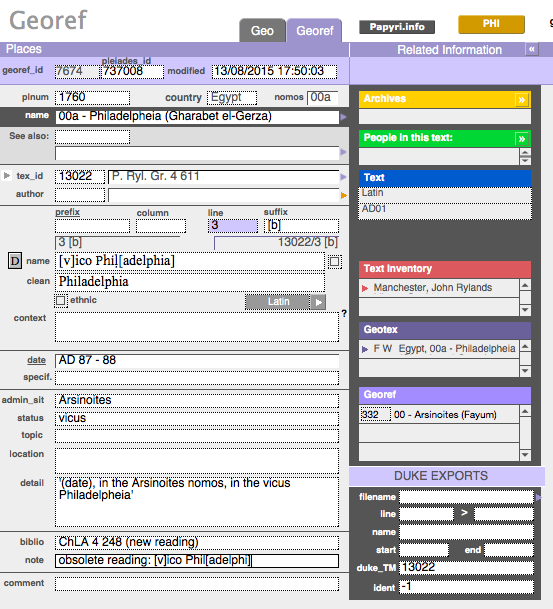
\includegraphics[width=\columnwidth]{EAGLE2016FullPaperVerreth-img003.png}
\caption{Philadelphia}
\label{fig:3}
\end{figure}
 

For every text in TM we try to give a reference to the most authoritative edition, where the user can find the best
and most up to date reading and interpretation of that text. As authoritative editions we preferably use CIL, Année
épigraphique and more recent major editions such as RIB, ILAlg, ICUR or I. Alex. Imp. Any corrections to the reading of
the toponym with regard to that edition are to be listed in the field Bibliography, while the obsolete reading is
recorded in the field Note. If the correction comes from one of the online full text databases, we add a reference to
the number of the text in that database.

A major problem is the dating of the texts. Unfortunately not every edition provides a date for each inscription.
Even if the scholar who publishes the text, has a fairly good idea of the century or range of time to which the text
might belong, it is not always mentioned explicitly in the edition. For every Latin text for which TM did not receive a
date from its partners, we added the broad range of 199 BC till AD 799, hoping that this dating will become more
refined in the future.

The third and final phase involves the context of the toponym. In the field Detail we give a plain translation of
the immediate phrase to which the toponym belongs. The translation should be a standardised as possible, with termini
technici preferably added in Latin, so that the users can easily search for them in the database; e.g. `\emph{Tiberius Iulius
Martialis son of Tiberius of (the tribus) Claudia from Savaria, soldier (miles) of legio XV Apollinaris}', `\emph{praefectus
Aegypti}', `\emph{cohors I Tungrorum}'. If the place is explicitly ascribed to a \emph{provincia} or a region, this \emph{provincia} is
listed in the field 'Administrative situation'. If a town is explicitly called an \emph{oppidum}, a \emph{vicus} or a \emph{civitas}, this
information is listed in the field Status. By adding this information in searchable fields we hope that the user can
start asking quite specific questions; e.g. the first and last attestation of a place in the sources; the periods in
which a town was called a \emph{colonia} or a \emph{municipium}; the places in which the `\emph{ala I Thracum Mauretana}' has been attested.

 TM is a relational database, which implies that is possible to get to the information from different angles. If
someone is studying a certain text, he can get a list of all toponyms mentioned in that text. On the other hand, if
someone is examining a certain place, he can find the list of all attestations for that place, in the order that he
wants. In some cases a scholar can have very specific questions, which are difficult to search through the online TM
search interface; it is quite well possible, however, that these questions can be easily answered in the more complex
Filemaker structure we have at our disposal; just contact us and we will try to solve the problem for you.

We are aware that this is a very succinct presentation of the new and exciting developments in Trismegistos Places,
but everybody interested is always more than welcome to ask for more information. Please feel free to provide us with
any addenda or corrigenda to the database you might have.

\bibliographystyle{sapauth-eng}
\bibliography{../../EAGLE}

\end{document}


